\parindent0pt
\makeatletter
\cxset{style12/.style={%
 chapter name=,
 chapter toc=true,
 chapter numbering=arabic,
 number font-size=HUGE,
 number font-family=rmfamily,
 number font-weight=bfseries,
 number before=,
 number dot=,
 number color= gray,
 number after=,
 number position=rightname,
 number float=left,
 number display=block,
 chapter font-family=sffamily,
 chapter font-weight=normalfont,
 chapter font-size=huge,
 chapter before=,
 chapter after=,
 chapter color={black!90},
 title beforeskip={\vspace*{0pt}},
 title afterskip={\vspace*{50pt}\par},
 title before=,
 title after={\par\vspace{20pt}\rule{\textwidth}{4pt}},
 title font-family=sffamily,
 title font-color=black!90,
 title font-weight=bfseries,
 title font-size=Huge,
 title font-shape=normal,
 title spaceout=none,
 chapter title width=.8\textwidth,
 chapter title align=left,
 chapter title text-align =left,
}}
\makeatother

\cxset{style12}
\chapter{Why Have They Become Mainstream so Quickly? }
\label{ch:style12}
This is a variation of Style 7, with only the lettering and the rule are thicker. In my opinion it looks better with a bit of color, so I have used a purple color with a gray.

\medskip
\begin{figure}[ht]
\centering
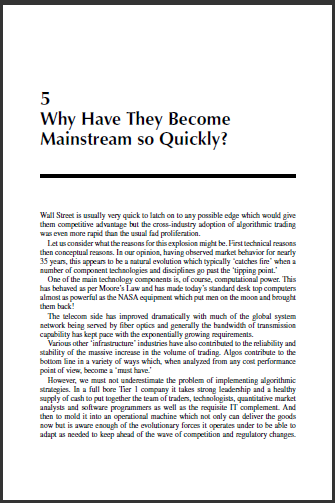
\includegraphics[width=0.35\textwidth]{./chapters/chapter12.png}
\caption{Style 12 sample from the book.}
\end{figure}
\lipsum[1]

